\section{Auswertung}
\label{sec:auswertung}

Die in der Auswertung verwendeten physikalischen Konstanten sind der Quelle \cite{CODATA} entnommen.

\subsection{Bestimmung der Hysteresekurve des verwendeten Elektromagneten}

Zunächst wird das Verhalten des verwendeten Elektromagneten untersucht. Dazu sind in Tabelle~\ref{tab:magnet} die gemessenen Feldstärken bei verschiedenen Strömen einer steigenden und einer fallenden Flanke aufgeführt. Lineare Interpolation dieser Werte liefert die in Abbildung~\ref{fig:magnet} dargestellte Kurve.
%
\begin{table}[H]
    \centering
    \caption{Feldstärken und Spulenströme der Messung.}
    \begin{tabular}{lcSSSr}
        \toprule
        & \multicolumn{1}{c}{Steigend} & \multicolumn{1}{c}{Fallend} \\
		{I [A]}  & {B [mT]}  & {B [mT]}                      \\
		\midrule
	  \SI{0}{}  & \SI{6}{}    & \SI{8}{} \\
    \SI{1}{}  & \SI{70}{}   & \SI{76}{} \\
		\SI{2}{}  & \SI{142}{}  & \SI{145}{} \\
		\SI{3}{}  & \SI{212}{}  & \SI{213}{} \\
		\SI{4}{}  & \SI{288}{}  & \SI{284}{} \\
    \SI{5}{}  & \SI{335}{}  & \SI{346}{} \\
    \SI{6}{}  & \SI{422}{}  & \SI{422}{} \\
    \SI{7}{}  & \SI{492}{}  & \SI{488}{} \\
    \SI{8}{}  & \SI{560}{}  & \SI{562}{} \\
    \SI{9}{}  & \SI{630}{}  & \SI{642}{} \\
    \SI{10}{} & \SI{698}{}  & \SI{733}{} \\
    \SI{11}{} & \SI{785}{}  & \SI{810}{} \\
    \SI{12}{} & \SI{873}{}  & \SI{890}{} \\
    \SI{13}{} & \SI{947}{}  & \SI{967}{} \\
    \SI{14}{} & \SI{1020}{} & \SI{1040}{} \\
    \SI{15}{} & \SI{1104}{} & \SI{1104}{} \\
		\bottomrule
	\end{tabular}
    \label{tab:magnet}
\end{table}
%
\begin{figure}[H]
    \centering
    \includegraphics[width=0.80\textwidth]{build/plot_magnetfeld.pdf}
    \caption{Darstellung der an beiden Flanken gemessenen Feldstärken in Abhängigkeit des Spulenstromes sowie der linearen Interpolation dieser Werte.}
    \label{fig:magnet}
\end{figure}

Es ergibt sich hierbei nach linearer Regression der Zusammenhang
%
\begin{equation}
  B(I)=\SI{73(2)}{\tesla\per\ampere}I-\SI{10(14)}{\tesla}.
  \label{eq:magnet}
\end{equation}

\subsection{Bestimmung des Dispersionsgebietes und des Auflösungsvermögens der Lummer-Gehrcke-Platte}

Die Lummer-Gehrcke-Platte ist mit einer Dicke von $\SI{4}{\milli\meter}$ und einer Länge von $\SI{120}{\milli\meter}$ angegeben. Die Brechungsindizes liegen bei den beiden relevanten Wellenlängen des Lichtes bei $n(\SI{643.8}{\nano\meter})=1,4567$ und $n(\SI{480}{\nano\meter})=1,4635$. Hieraus lässt sich das Auflösungsvermögen $A$ über den Zusammenhang
%
\begin{equation}
  A=\frac{\lambda}{\mathup{\Delta}\lambda_D}=\frac{L}{\lambda}(n^2-1)
  \label{eq:Auflösungsvermögen}
\end{equation}
%
mit Hilfe des Dispersionsgebietes bestimmen. Es ergeben sich die in Tabelle~\ref{tab:platte} aufgeführten Werte.
%
\begin{table}[H]
    \centering
    \caption{Dispersionsgebiet und Auflösungsvermögen der Lummer-Gehrcke-Platte für die verschiedenen Wellenlängen.}
    \begin{tabular}{SSSS}
        \toprule
        \multicolumn{1}{c}{Wellenlänge} & \multicolumn{1}{c}{Dispersionsgebiet } & \multicolumn{1}{c}{Auflösungsvermögen} \\
		{ $\lambda$ [nm]}  & {$\mathup{\Delta}\lambda_D$ [pm]}  & {A} \\
		\midrule
	  \SI{643,8}{}  & \SI{48,91}{}    & \SI{209128}{} \\
    \SI{480}{}  & \SI{26,95}{}   & \SI{285458}{} \\
		\bottomrule
	\end{tabular}
    \label{tab:platte}
\end{table}
%

\subsection{Zur Berechnung des Lande-Faktors}

Zur Bestimmung des Lande-Faktors werden die mit einer Digitalkamera aufgenommenen Bilder des Interferenzspektrums ausgewertet. Um die Abstände der Maxima zu bestimmen werden mit Hilfe eines Grafikprogrammes in die nach Augenmaß subjektiv vermutete Mitte der einzelnen Maxima Linien eingezeichnet. Der Abstand $\mathup{\Delta} s$ zwischen diesen Linien wird dann in pixel für die Aufnahmen ohne B-Feld ausgemessen. Für die Aufnahmen bei eingeschaltetem Magnetfeld werden die Abstände $\delta s$ zwischen den Aufspaltungen auf gleiche Weise ausgemessen. Im Folgenden sind diese Werte in Tabellen mit den dazugehörigen Aufnahmen aufgeführt. Aus den Messwerten lässt sich nun der Faktor $\delta\lambda$ bestimmen:
%
\begin{equation}
  \delta\lambda=\frac{1}{2}\frac{\delta s}{\mathup{\Delta} s}\mathup{\Delta}\lambda_D.
  \label{eq:dlambda}
\end{equation}
%
Das Dispersionsgebiet kann dabei dem vorigen Kapitel entnommen werden. Um den Lande-Faktor zu berechnen wird der Zusammenhang
%
\begin{equation}
  |\mathup{\Delta}E|=|\mathup{\Delta m}|g\mu_BB
  \label{eq:dE}
\end{equation}
%
verwendet. Hierbei ist $\mu_B$ das Bohrsche Magneton und $\mathup{\Delta}m$ der Unterschied in der Magnetquantenzahl für den jeweiligen Übergang. Aus dem Zusammenhang $E=\sfrac{hc}{\lambda}$ ergibt sich durch Ableiten
%
\begin{equation}
  \frac{\partial E}{\partial\lambda}=-\frac{hc}{\lambda^2}.
  \label{eq:partE}
\end{equation}
%
Hieraus folgt schließlich unter der Bedingung $|\mathup{\Delta}E|\approx|\mathup{\Delta\lambda_D}|\sfrac{hc}{\lambda²}$ mit Gleichung~\eqref{eq:dE} für $|\mathup{\Delta}m|=1$ als Lande-Faktor:
%
\begin{equation}
  g=\frac{hc\delta\lambda}{\lambda^2\mu_BB}\; .
  \label{eq:lande}
\end{equation}

\subsection{Messung der Wellenlängenunterschiede und Bestimmung des Lande-Faktors}

Das Interferenzmuster für die $\sigma$-Linie des roten Lichtes ($\SI{643,8}{\nano\meter}$) ist in der Abbildung~\ref{fig:rotsigma} ohne anliegendes Magnetfeld und in der Abbildung~\ref{fig:rotsigma_b} mit anliegendem Magnetfeld dargestellt. Die gemessenen Abstände sind in Tabelle~\ref{tab:rotsigma} aufgeführt.

\begin{figure}[H]
    \centering
    \includegraphics[width=0.75\textwidth]{figure/sigma_rot_bfeld_bearbeitet.jpg}
    \caption{Darstellung der Abstände der Interferenzmaxima in der Kameraaufnahme für die rote $\sigma$-Linie bei eingeschaltetem Magnetfeld.}
    \label{fig:rotsigma_b}
\end{figure}
%
\begin{figure}[h]
    \centering
    \includegraphics[width=0.75\textwidth]{figure/sigma_rot_bearbeitet.jpg}
    \caption{Darstellung der Abstände der Interferenzmaxima in der Kameraaufnahme für die rote $\sigma$-Linie bei ausgeschaltetem Magnetfeld.}
    \label{fig:rotsigma}
\end{figure}
%
\begin{table}[H]
    \centering
    \caption{Abstände der Interferenzmaxima (in pixel), die daraus bestimmten $\delta\lambda$ sowie die berechneten Lande-Faktoren für die rote $\sigma$-Linie.}
    \begin{tabular}{SSSSS}
        \toprule
    \multicolumn{1}{c}{Ordnung}  & \multicolumn{1}{c}{Abstand} & \multicolumn{1}{c}{Abstand mit B-Feld} & & \multicolumn{1}{c}{Lande-Faktor}\\
		{}  & {$\mathup{\Delta}s$ [px]}  & {$\delta s$ [px]} & {$\delta\lambda$ [pm]} & g \\
		\midrule
    \SI{0}{}  & \SI{285}{}  & \SI{171}{} & \SI{14,67}{} & \SI{1.114}{} \\
    \SI{1}{}  & \SI{290}{}  & \SI{144}{} & \SI{12,14}{} & \SI{0.922}{} \\
		\SI{2}{}  & \SI{251}{}  & \SI{132}{} & \SI{12,86}{} & \SI{0.976}{} \\
    \SI{3}{}  & \SI{241}{}  & \SI{114}{} & \SI{11,56}{} & \SI{0.878}{} \\
    \SI{4}{}  & \SI{218}{}  & \SI{104}{} & \SI{11,66}{} & \SI{0.886}{} \\
    \SI{5}{}  & \SI{212}{}  & \SI{110}{} & \SI{12,68}{} & \SI{0.963}{} \\
    \SI{6}{}  & \SI{202}{}  & \SI{100}{} & \SI{12,10}{} & \SI{0.919}{} \\
    \SI{7}{}  & \SI{182}{}  & \SI{92}{}  & \SI{12,36}{} & \SI{0.939}{} \\
    \SI{8}{}  & \SI{175}{}  & \SI{94}{}  & \SI{13,13}{} & \SI{0.997}{} \\
    \SI{9}{}  & \SI{179}{}  & \SI{96}{}  & \SI{13,11}{} & \SI{0.996}{} \\
    \SI{10}{} & \SI{173}{}  & \SI{90}{}  & \SI{12,72}{} & \SI{0.966}{} \\
    \SI{11}{} & \SI{173}{}  & \SI{83}{}  & \SI{11,73}{} & \SI{0.891}{} \\
    \bottomrule
	\end{tabular}
    \label{tab:rotsigma}
\end{table}
%
Die Messung der roten $\sigma$-Linie wird bei einer Stromstärke von $\SI{10}{\ampere}$ durchgeführt, sodass sich aus der Hysterese nach Gleichung~\eqref{eq:magnet} ein magnetischer Fluss von etwa $\SI{0.717}{\tesla}$ ableiten lässt. Es ergibt sich hier als Mittelwert für den Lande-Faktor $0.91\,\pm\, 0.06$.

%
\begin{figure}[h]
    \centering
    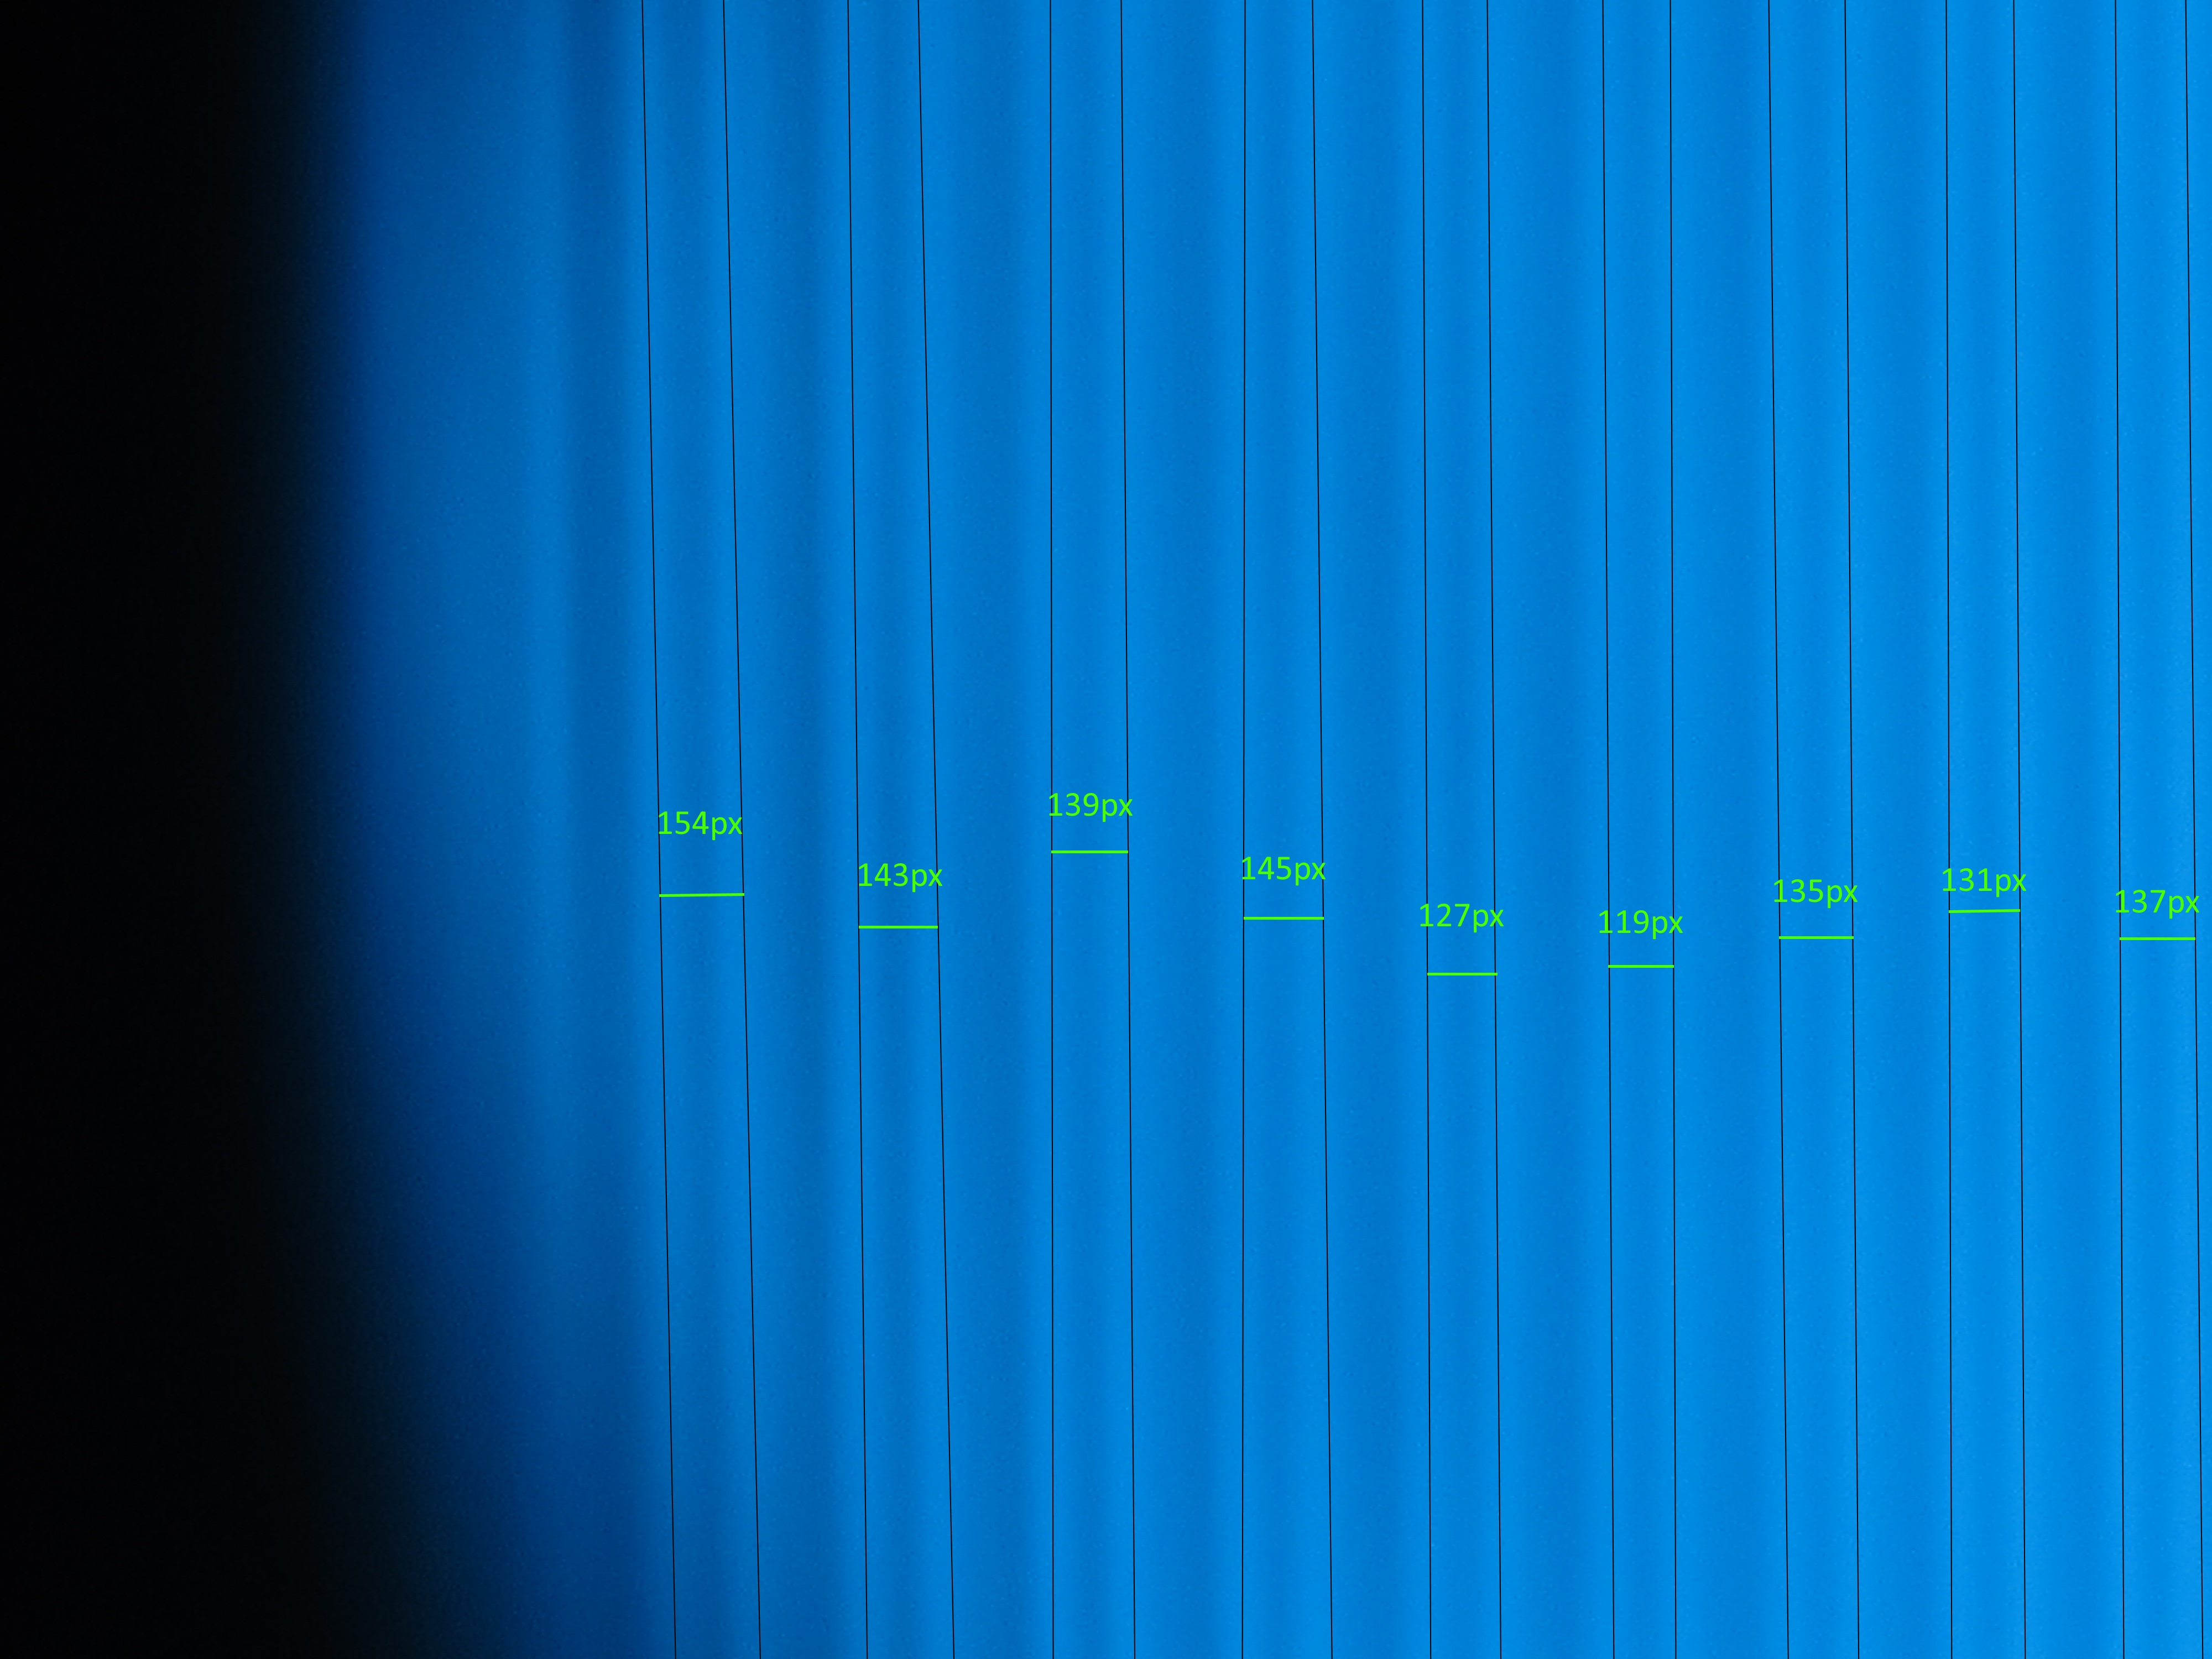
\includegraphics[width=0.75\textwidth]{figure/blausigma_bfeld_bearbeitet.jpg}
    \caption{Darstellung der Abstände der Interferenzmaxima in der Kameraaufnahme für die blaue $\sigma$-Linie bei eingeschaltetem Magnetfeld.}
    \label{fig:blausigma_b}
\end{figure}
%
\begin{figure}[h]
    \centering
    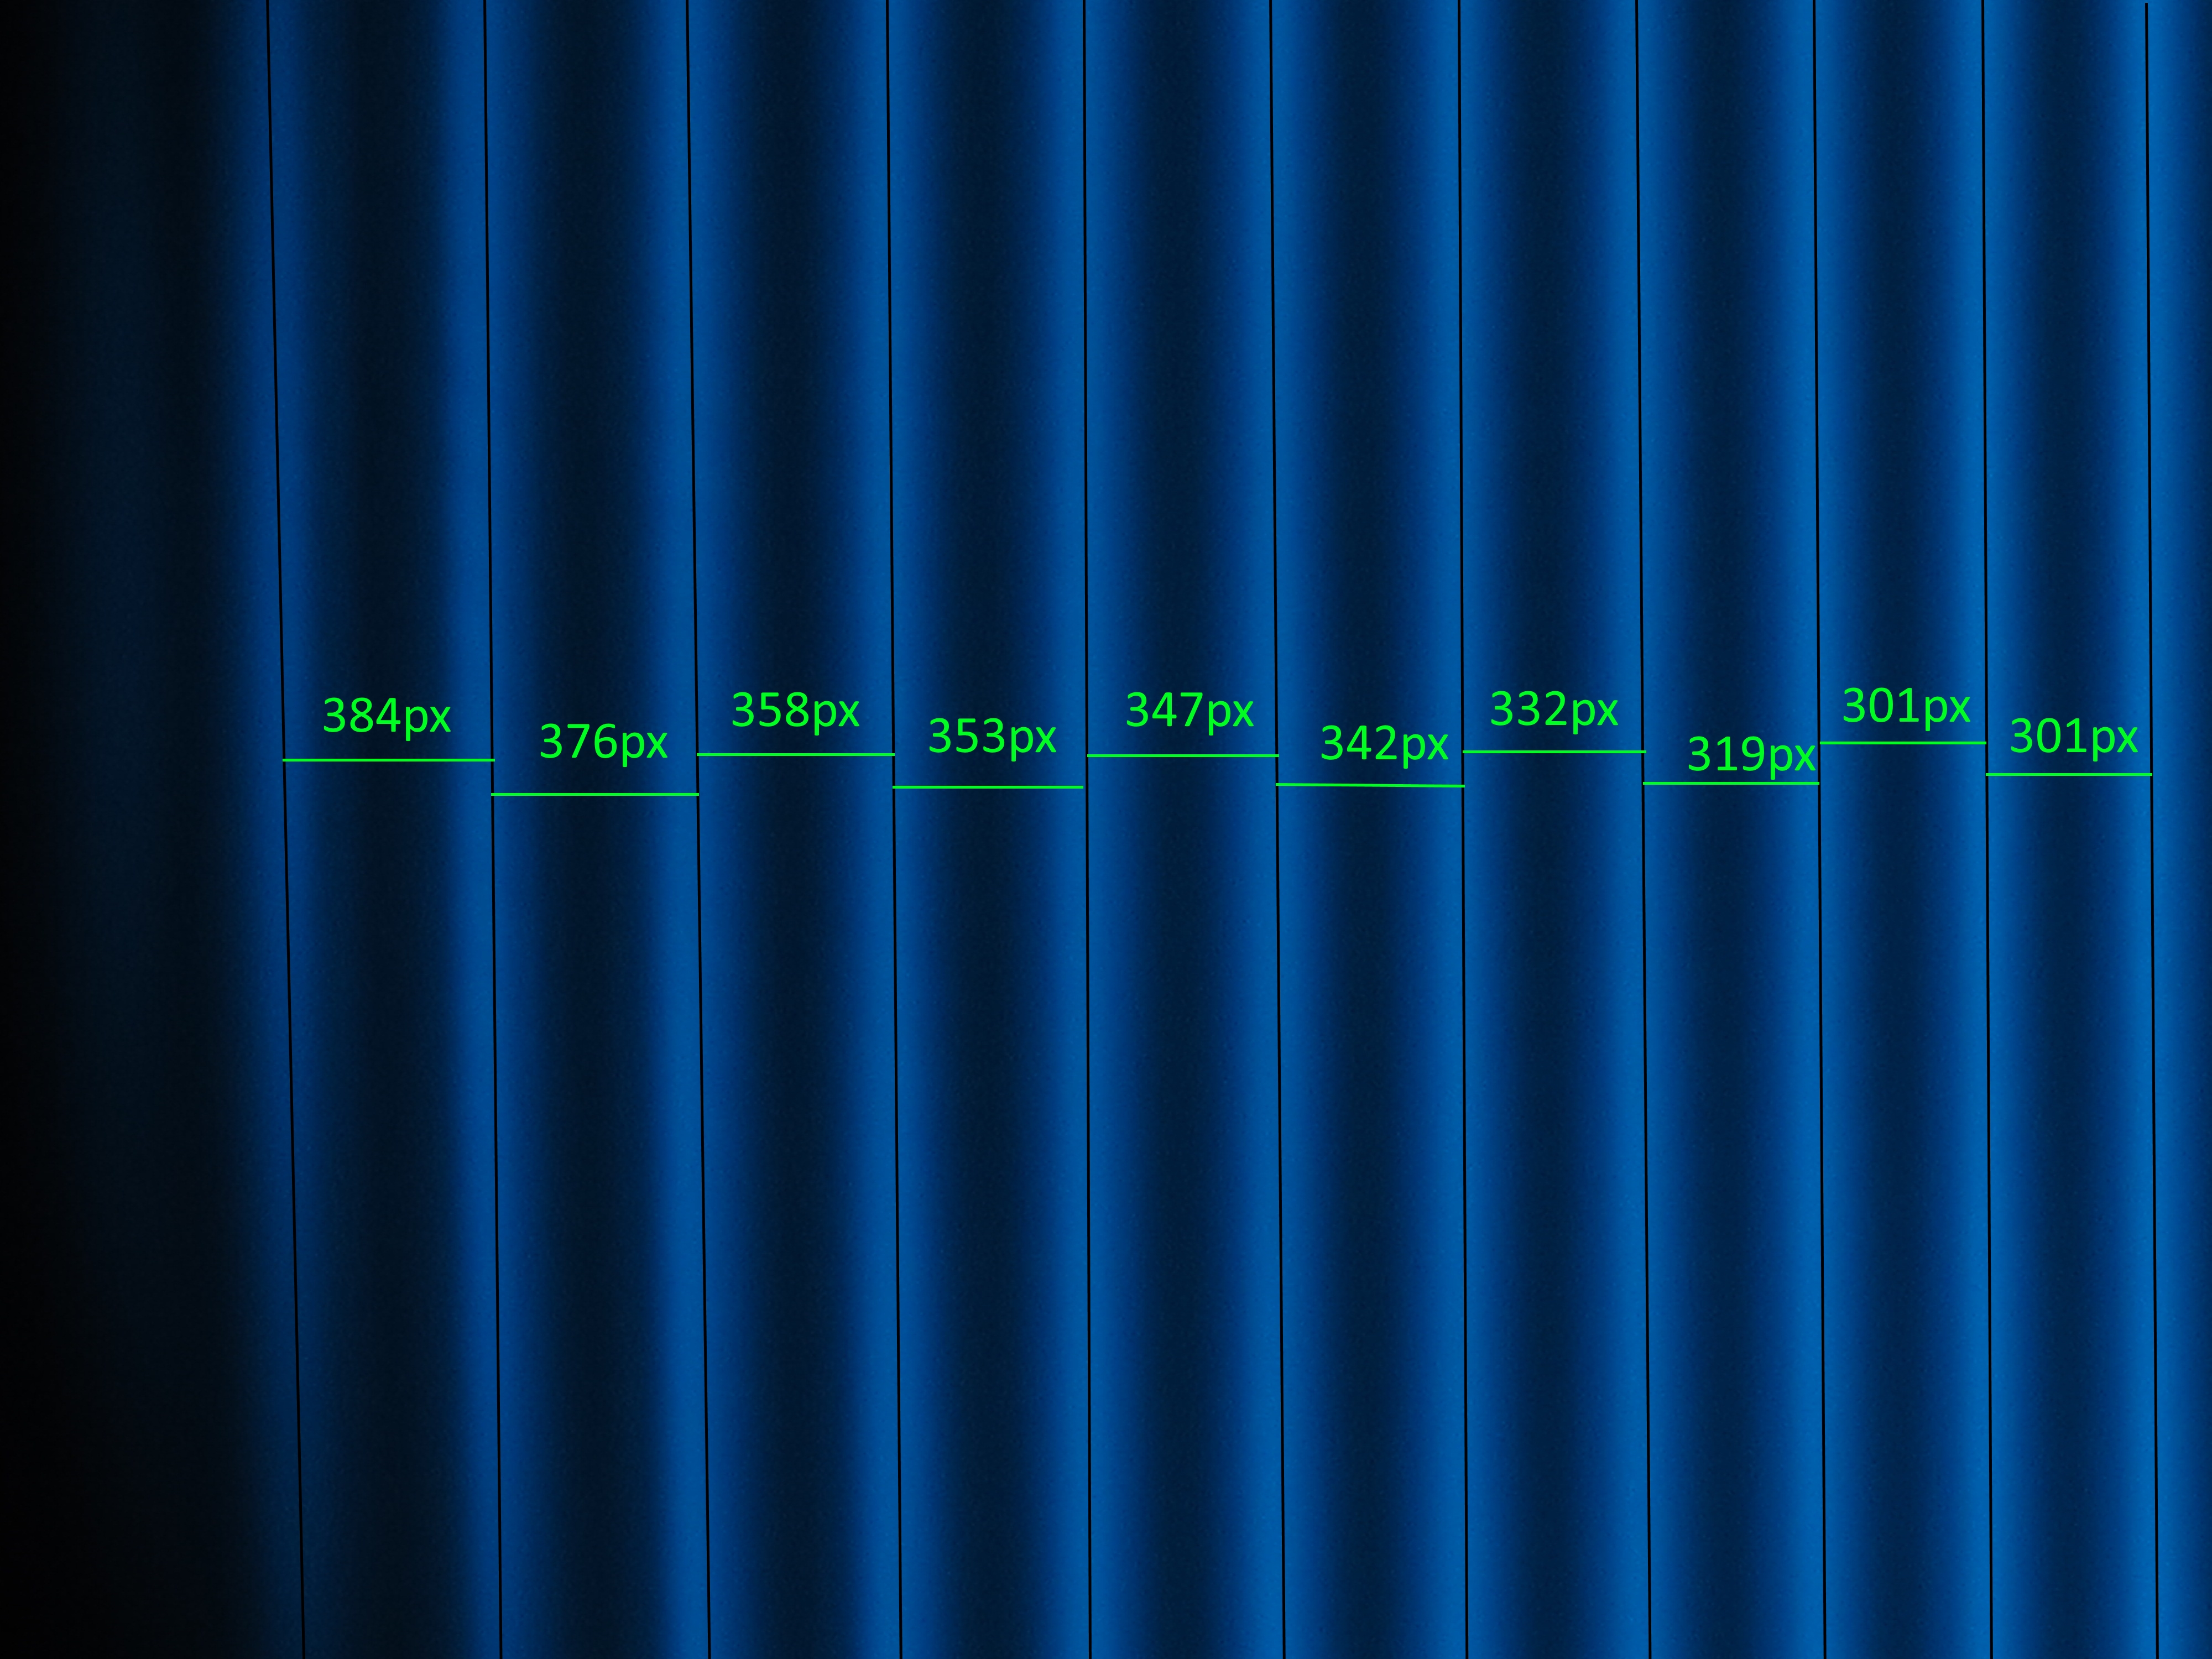
\includegraphics[width=0.75\textwidth]{figure/blausigma_bearbeitet.jpg}
    \caption{Darstellung der Abstände der Interferenzmaxima in der Kameraaufnahme für die blaue $\sigma$-Linie bei ausgeschaltetem Magnetfeld.}
    \label{fig:blausigma}
\end{figure}
%
\begin{table}[H]
    \centering
    \caption{Abstände der Interferenzmaxima (in pixel), die daraus bestimmten $\delta\lambda$ sowie die berechneten Lande-Faktoren für die blaue $\sigma$-Linie.}
    \begin{tabular}{SSSSS}
        \toprule
    \multicolumn{1}{c}{Ordnung}  & \multicolumn{1}{c}{Abstand} & \multicolumn{1}{c}{Abstand mit B-Feld} & & \multicolumn{1}{c}{Lande-Faktor}\\
		{}  & {$\mathup{\Delta}s$ [px]}  & {$\delta s$ [px]} & {$\delta\lambda$ [pm]} & g \\
		\midrule
    \SI{0}{}  & \SI{384}{}  & \SI{154}{} & \SI{5.404}{} & \SI{1.424}{} \\
    \SI{1}{}  & \SI{376}{}  & \SI{143}{} & \SI{5.125}{} & \SI{1.350}{} \\
		\SI{2}{}  & \SI{358}{}  & \SI{139}{} & \SI{5.232}{} & \SI{1.379}{} \\
    \SI{3}{}  & \SI{353}{}  & \SI{145}{} & \SI{5.535}{} & \SI{1.459}{} \\
    \SI{4}{}  & \SI{347}{}  & \SI{127}{} & \SI{4.932}{} & \SI{1.3}{} \\
    \SI{5}{}  & \SI{342}{}  & \SI{119}{} & \SI{4.689}{} & \SI{1.236}{} \\
    \SI{6}{}  & \SI{332}{}  & \SI{135}{} & \SI{5.479}{} & \SI{1.444}{} \\
    \SI{7}{}  & \SI{319}{}  & \SI{131}{} & \SI{5.534}{} & \SI{1.458}{} \\
    \SI{8}{}  & \SI{301}{}  & \SI{137}{} & \SI{6.133}{} & \SI{1.616}{} \\
    \bottomrule
	\end{tabular}
    \label{tab:blausigma}
\end{table}
%
Die Messung der blauen $\sigma$-Linie wird bei einer Stromstärke von $\SI{5}{\ampere}$ durchgeführt, sodass sich aus der Hysterese nach Gleichung~\eqref{eq:magnet} ein magnetischer Fluss von etwa $\SI{0.353}{\tesla}$ ableiten lässt. Es ergibt sich hier als Mittelwert für den Lande-Faktor $1.4\,\pm\, 0.1$.
%
\begin{figure}[h]
    \centering
    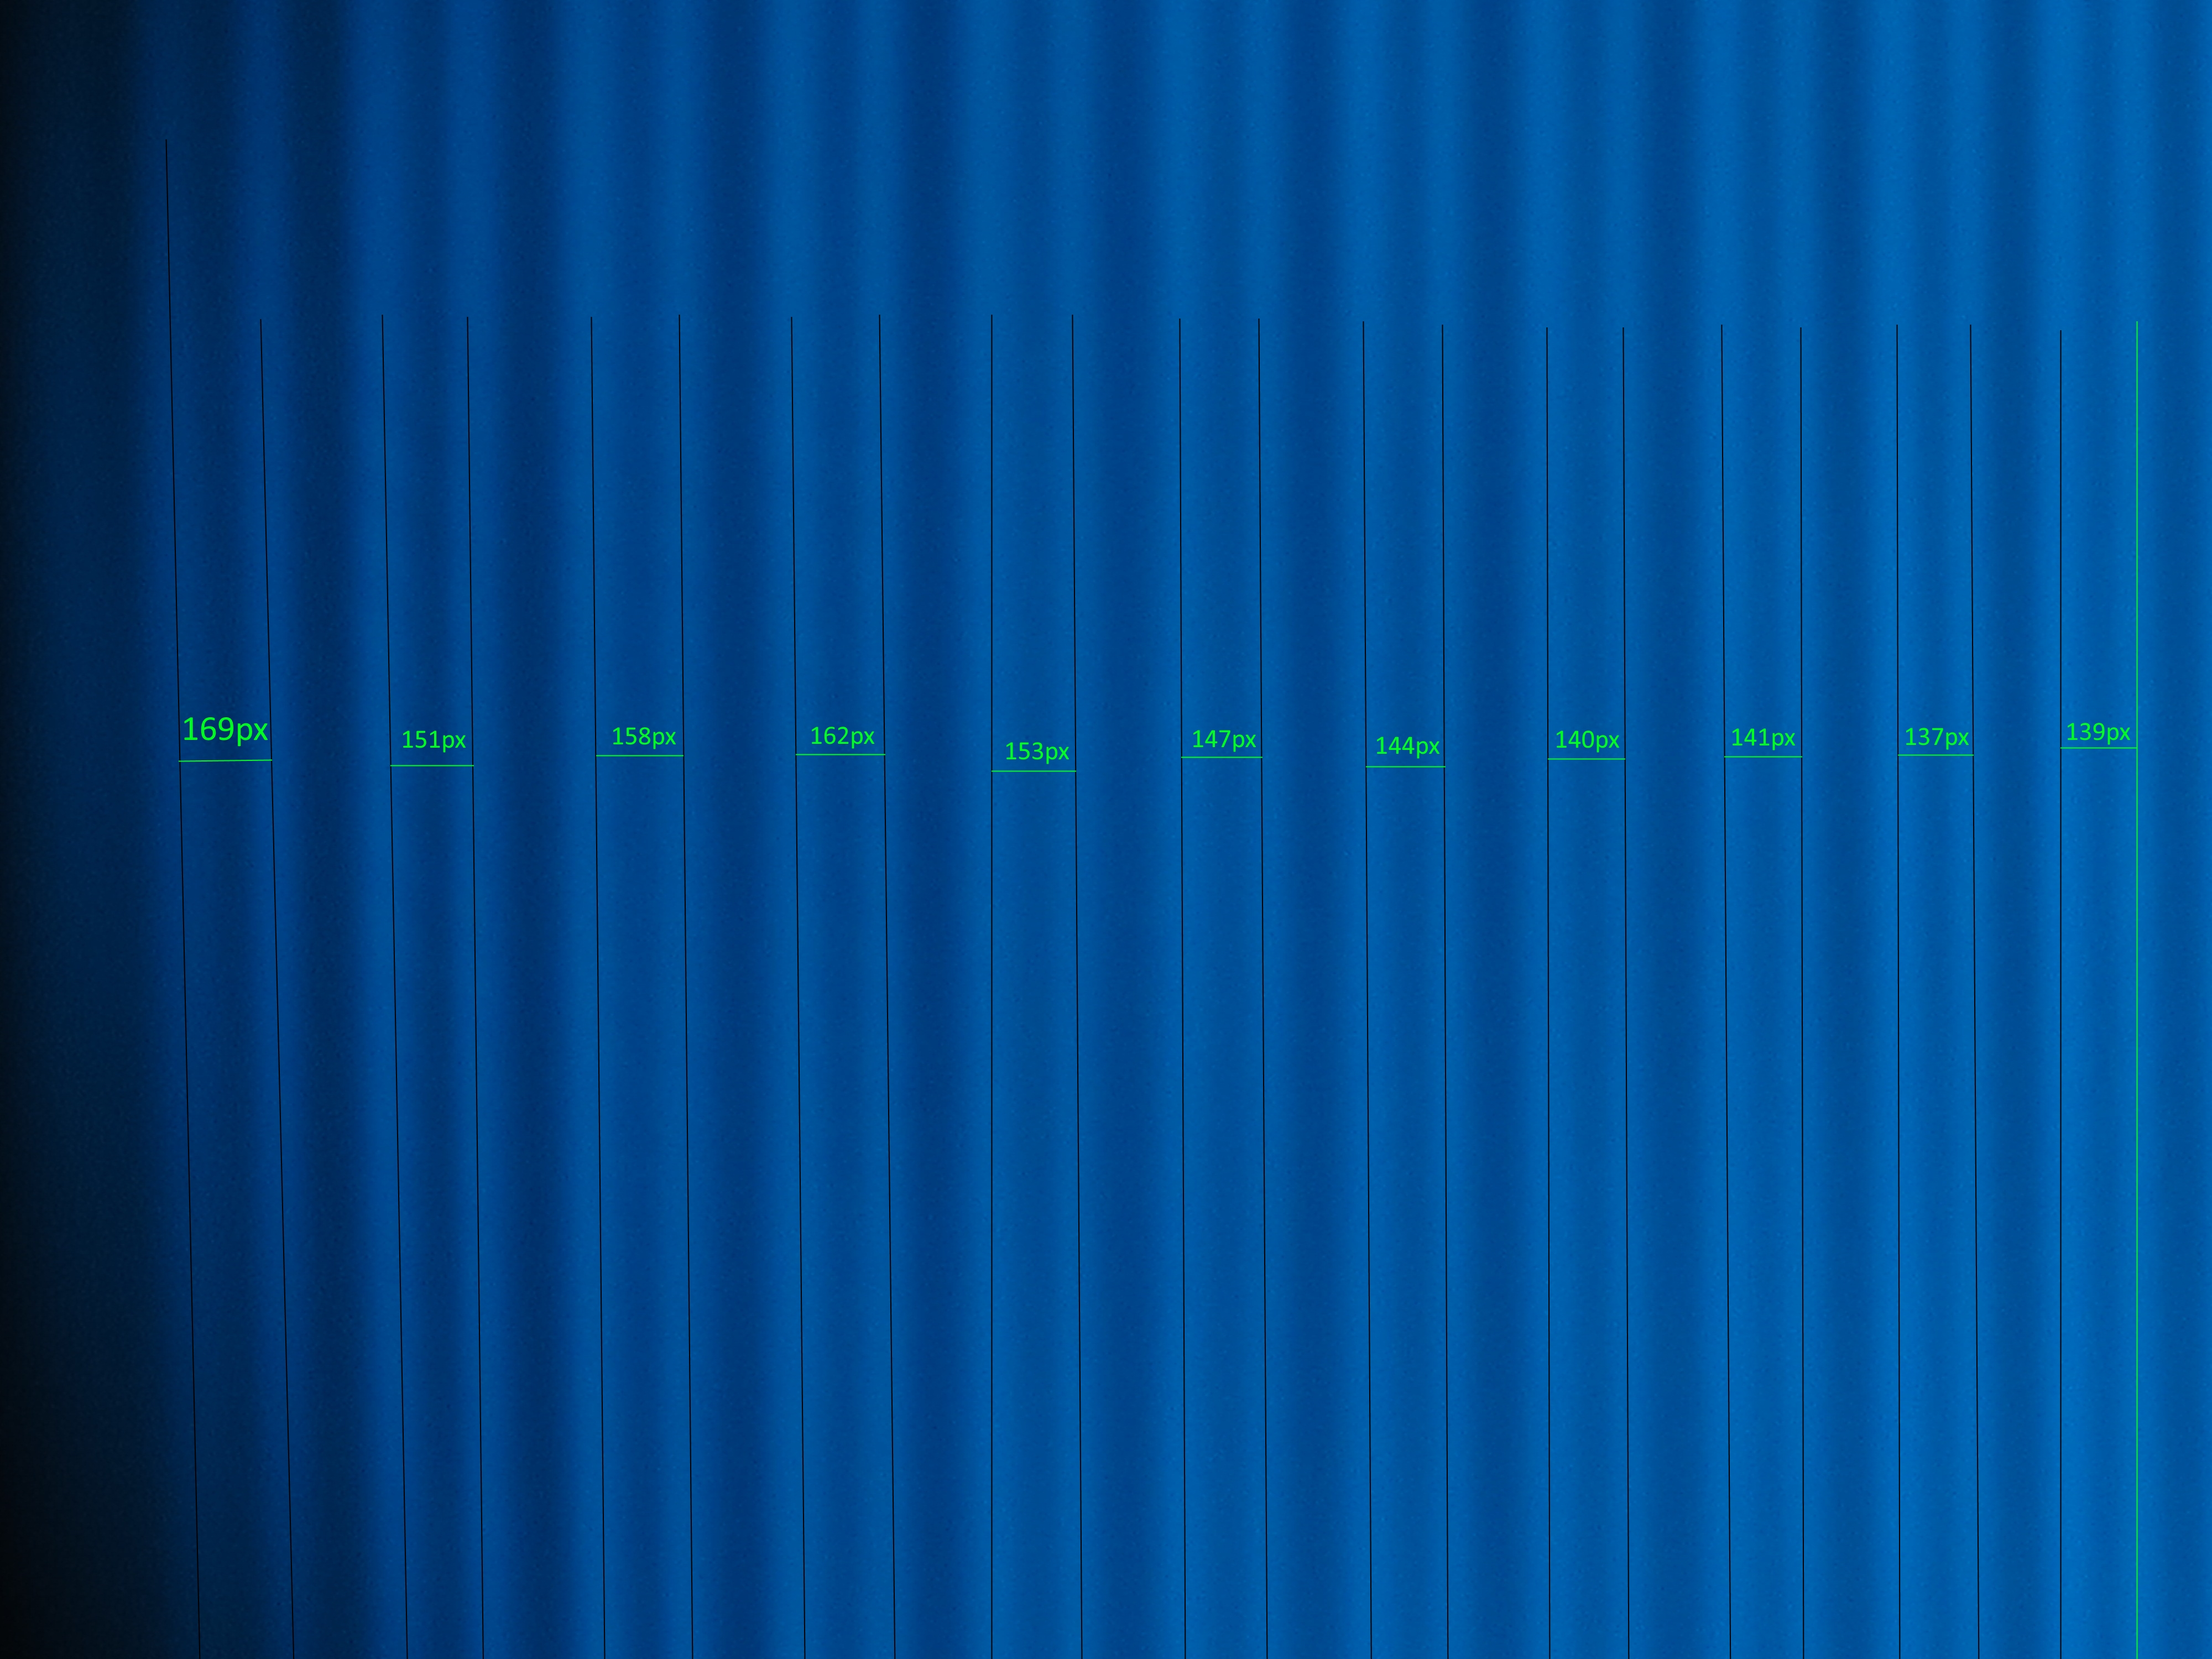
\includegraphics[width=0.75\textwidth]{figure/blaupi_bfeld_bearbeitet.jpg}
    \caption{Darstellung der Abstände der Interferenzmaxima in der Kameraaufnahme für die blaue $\pi$-Linie bei eingeschaltetem Magnetfeld.}
    \label{fig:blaupi_b}
\end{figure}
%
\begin{figure}[h]
    \centering
    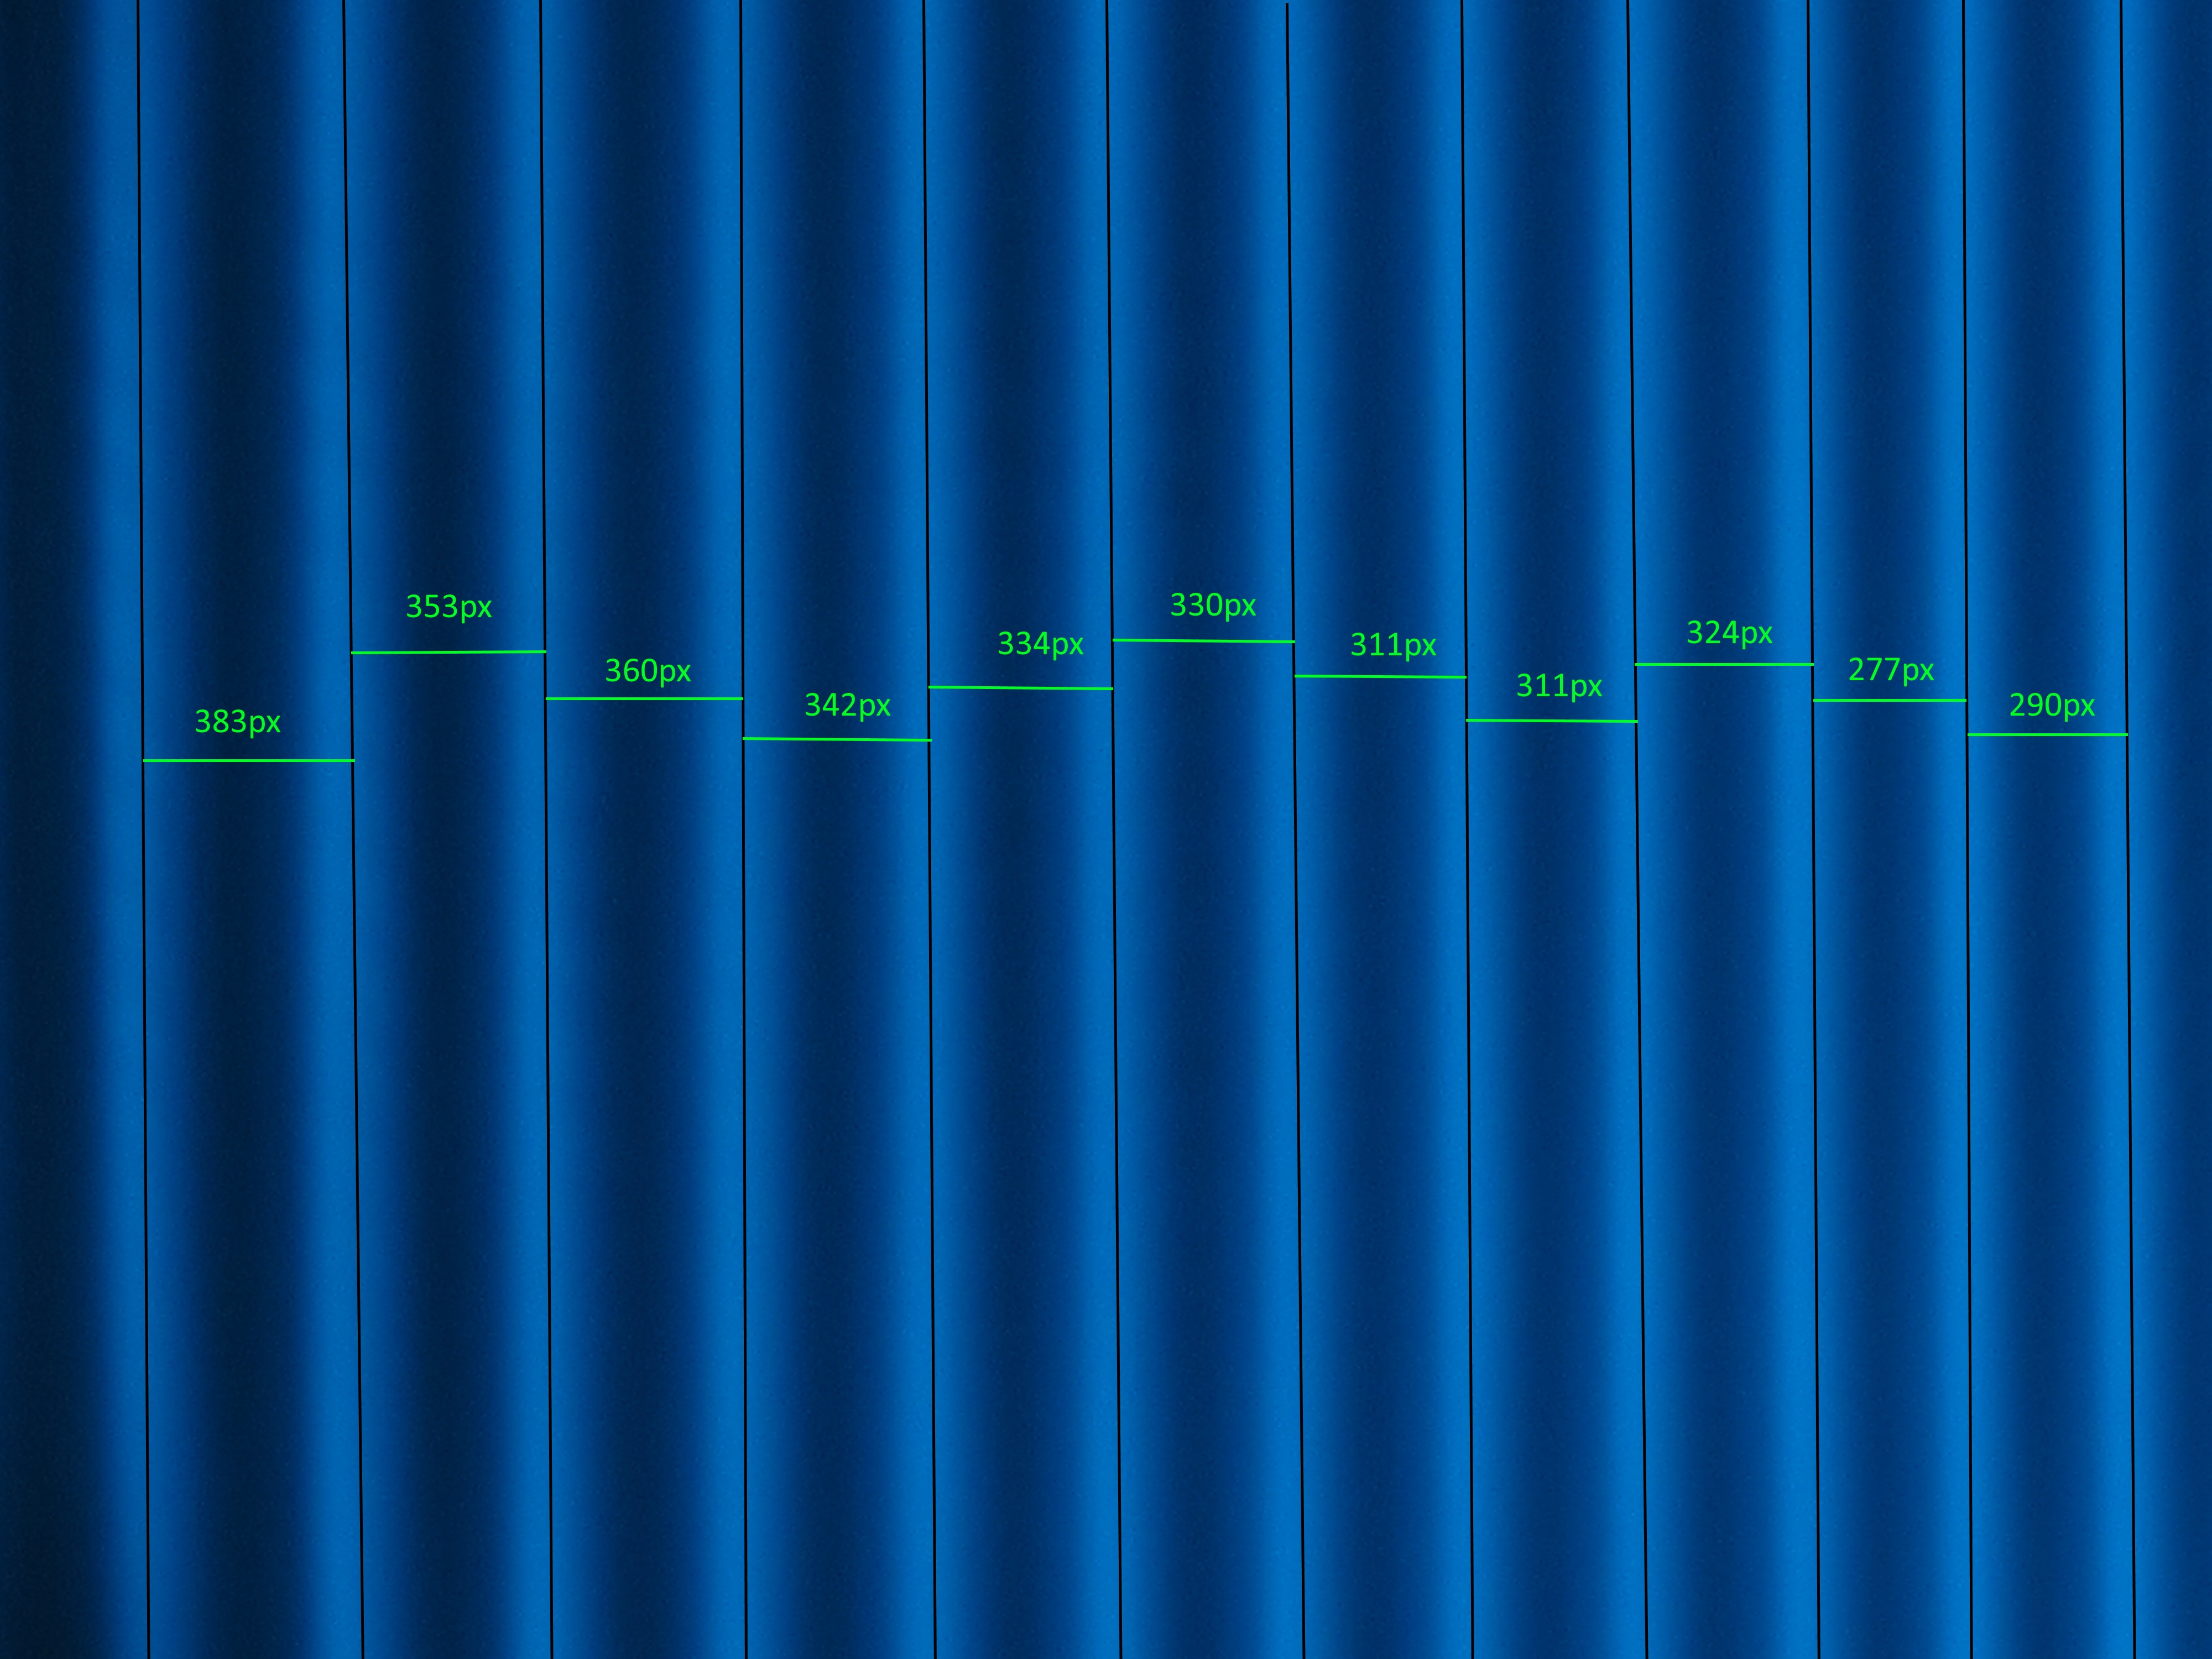
\includegraphics[width=0.75\textwidth]{figure/blaupi_bearbeitet.jpg}
    \caption{Darstellung der Abstände der Interferenzmaxima in der Kameraaufnahme für die blaue $\pi$-Linie bei ausgeschaltetem Magnetfeld.}
    \label{fig:blaupi}
\end{figure}
%
\begin{table}[H]
    \centering
    \caption{Abstände der Interferenzmaxima (in pixel), die daraus bestimmten $\delta\lambda$ sowie die berechneten Lande-Faktoren für die blaue $\pi$-Linie.}
    \begin{tabular}{SSSSS}
        \toprule
    \multicolumn{1}{c}{Ordnung}  & \multicolumn{1}{c}{Abstand} & \multicolumn{1}{c}{Abstand mit B-Feld} & & \multicolumn{1}{c}{Lande-Faktor}\\
		{}  & {$\mathup{\Delta}s$ [px]}  & {$\delta s$ [px]} & {$\delta\lambda$ [pm]} & g \\
		\midrule
    \SI{0}{}   & \SI{383}{}  & \SI{169}{} & \SI{5.946}{} & \SI{0.511}{} \\
    \SI{1}{}   & \SI{353}{}  & \SI{151}{} & \SI{5.764}{} & \SI{0.496}{} \\
    \SI{2}{}   & \SI{360}{}  & \SI{158}{} & \SI{5.914}{} & \SI{0.508}{} \\
    \SI{3}{}   & \SI{342}{}  & \SI{162}{} & \SI{6.383}{} & \SI{0.549}{} \\
    \SI{4}{}   & \SI{224}{}  & \SI{153}{} & \SI{9.204}{} & \SI{0.791}{} \\
    \SI{5}{}   & \SI{330}{}  & \SI{147}{} & \SI{6.002}{} & \SI{0.516}{} \\
    \SI{6}{}   & \SI{311}{}  & \SI{144}{} & \SI{6.239}{} & \SI{0.536}{} \\
    \SI{7}{}   & \SI{311}{}  & \SI{140}{} & \SI{6.066}{} & \SI{0.521}{} \\
    \SI{8}{}   & \SI{324}{}  & \SI{141}{} & \SI{5.864}{} & \SI{0.504}{} \\
    \SI{9}{}   & \SI{277}{}  & \SI{137}{} & \SI{6.665}{} & \SI{0.573}{} \\
    \SI{10}{}  & \SI{290}{}  & \SI{139}{} & \SI{6.459}{} & \SI{0.555}{} \\
    \bottomrule
	\end{tabular}
    \label{tab:blaupi}
\end{table}
%
Die Messung der blauen $\pi$-Linie wird bei einer Stromstärke von $\SI{15}{\ampere}$ durchgeführt, sodass sich aus der Hysterese nach Gleichung~\eqref{eq:magnet} ein magnetischer Fluss von etwa $\SI{1.08}{\tesla}$ ableiten lässt. Es ergibt sich hier als Mittelwert für den Lande-Faktor $0.55\,\pm\, 0.08$.
